\chapter{Kernel Density Estimation}
\section{KDE in 1 Dimension}
\label{sec:1d}
Let's first consider the one-dimensional case. Fig.~\ref{fig:1d_hist} shows a histogram for a series of observations drawn from an exponentially-modified Gaussian distribution. We choose this distribution to illustrate the impact of non-Gaussianity (in particular skewness) on the resulting estimates of the underlying probability distribution. The true probability distribution function is shown as a black line in Fig.~\ref{fig:1d_hist}. The remaining lines in Fig.~\ref{fig:1d_hist} show the resulting kernel density estimates using a Gaussian kernel with a range of bandwidth values. We can qualitatively see that a bandwidth of 0.53 results in an estimate that closely resembles the true probability distribution, while a value of 0.1 is too narrow (overfitting/high variance) and 3 is too wide (underfitting/high bias).

\begin{figure}
    \centering
    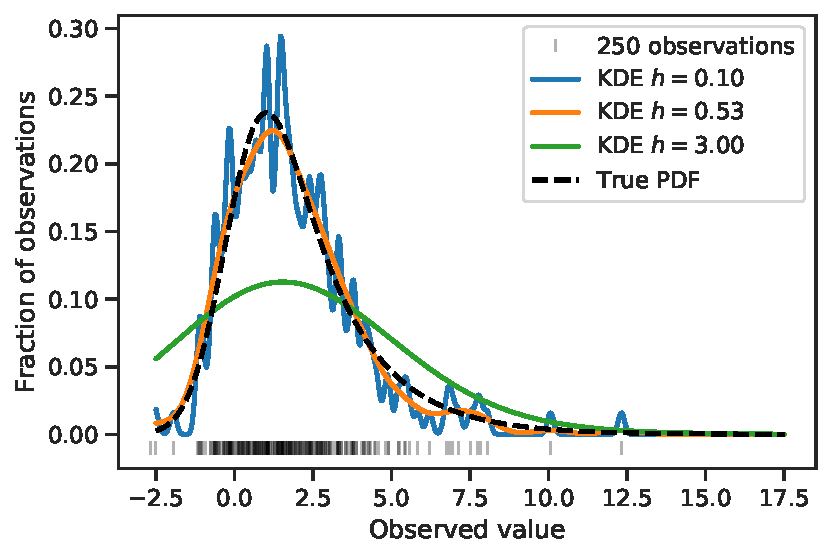
\includegraphics{figures/snemo_kde/1d_hist_example.pdf}
    \caption{Example of a kernel density estimate of a 1-dimensional, non-Gaussian distribution. The ticks represent the $n=250$ observations drawn from the true distribution shown with the black dashed line. The blue, orange, and green lines represent KDEs with increasing bandwidth sizes.}
    \label{fig:1d_hist}
\end{figure}

There are some general rules-of-thumb for selecting an optimal bandwidth; for example, Silverman's rule of thumb:
$$h= 0.9\times\min\left(\hat{\sigma}, \frac{\textrm{IQR}}{1.34}\right) \times n^{-1/5}$$
where $\hat{\sigma}$ is the standard deviation of the sample, $\textrm{IQR}$ is the interquartile range of the sample, and $n$ is the number of data points in the sample \citep{silverman_density_1986}. This rule can perform quite well in most circumstances. However, these types of rules-of-thumb generalize quite poorly when the data is highly non-Gaussian (e.g. multi-modal distributions) or when the dimensionality of the data is high.

Another way to find the best bandwidth parameter is to try several values of the parameter and compare the results via some metric. A commonly used method for performing this type of evaluation is $k$-fold cross-validation. In $k$-fold cross-validation, we split the sample into $k$ groups. We then hold one of these groups out and train the model on the examples in the remaining $k-1$ groups. The model is then evaluated on the examples in the held-out set. This process is repeated until each example in the data set has been used in the training and validation. The overall model evaluation is then usually taken to be the mean of the evaluation metrics found in each of the cross-validation rounds, and the standard deviation of these metrics can be used to estimate the uncertainty on that metric.

Using this technique on our toy example from above, we find an optimal bandwidth of 0.53, as evidenced by the maximum at this point in Fig.~\ref{fig:1d_bandwidth_opt}, plotting the total log probability of the $k$-folds as a function of bandwidth parameter. This differs from the location of the rule-of-thumb estimate; however, the difference in the average log-likelihoods of the data under a model with the rule-of-thumb bandwidth and the data under a model with the cross-validation selected bandwidth is small. Because the rule-of-thumb estimates have many downsides (and indeed are not well-defined in multiple dimensions) and because cross-validation gives us bandwidths that perform equally well or better, we proceed with the cross-validation bandwidth selection.

\begin{figure}
    \centering
    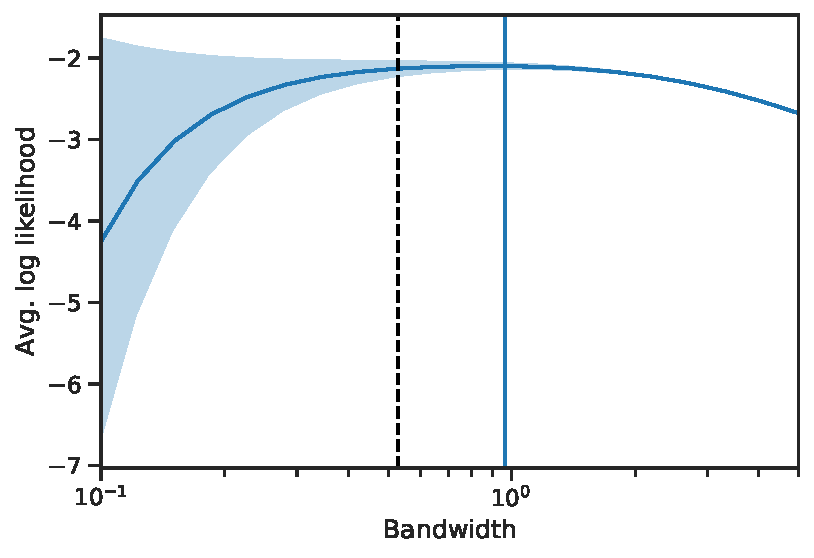
\includegraphics{figures/snemo_kde/1d_bandwidth_example.pdf}
    \caption{Results from 5-fold cross-validation for the example distribution and data shown in Fig.~\ref{fig:1d_hist}. The blue line and shading show the mean and standard deviation of the normalized scores from all of the cross-validation subsets. The vertical blue line shows the location of the maximum score. The dashed black line shows the location of the Silverman's rule-of-thumb estimate for the optimal bandwidth.}
    \label{fig:1d_bandwidth_opt}
\end{figure}

\section[KDE in d Dimensions]{Appendix: KDE in $d$ Dimensions}
\label{sec:2d}
The case in $d>1$ is quite similar to the 1-dimensional case. The kernel, though, is now in $d$ dimensions, and as such, the bandwidth is no longer a single parameter but a $d\times d$ symmetric matrix describing the bandwidth in each dimension along with the correlations between dimensions. The higher-dimensional case is further complicated by the so-called ``curse of dimensionality", where the sparseness of the data in the higher dimensional space causes the density estimate to converge more slowly. We will explore this first detail with a similar toy model to that used in \ref{sec:1d} but in 2 dimensions for ease of visualization.

Consider a 2-dimensional sample drawn from a bivariate Gaussian distribution with mean $\bm{\mu}$ and covariance $\bm{\Sigma}$ (i.e. $(y_1, y_2)\sim\mathcal{N}(\bm{\mu}, \bm{\Sigma})$) and then consider a non-linear transformation to that sample, transforming $y_2$ to $z_2 = \exp(y_2)$. 

This example joint distribution is correlated and nonlinear, and as such works as a good test of the power and limitations of our methodology. We start by making estimates width a Gaussian kernel for a range of bandwidths as we did in the 1-dimensional case, giving us the results shown in Fig.~\ref{fig:2d_scatter_unscaled}. However, the standard \verb|sklearn| implementation of the kernel density estimator only allows for the a kernel with a covariance matrix  proportional to the identity matrix, so in our $k$-fold cross-validation, we are tuning a single bandwidth parameter $h$.

\begin{figure}
    \centering
    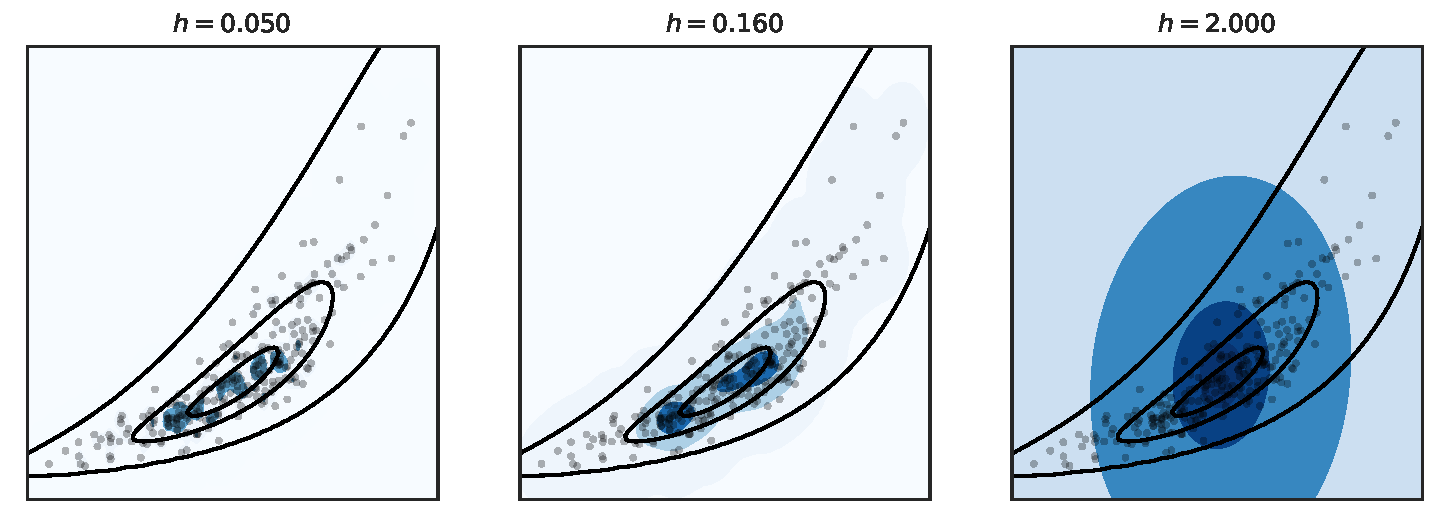
\includegraphics[width=0.9\textwidth]{figures/snemo_kde/2d_scatter_no_scaling.pdf}
    \caption{Example kernel density estimates in 2 dimensions for a joint probability distribution that is correlated and non-Gaussian. The $n=250$ data points are shown as black dots. The black contour lines show the true 1, 2, and 3 $\sigma$ contours, while the fading shades of blue show the 1, 2, and 3 $\sigma$ estimates of the KDE. In each of these examples, we assume a Gaussian kernel with no covariance terms.}
    \label{fig:2d_scatter_unscaled}
\end{figure}

We can see in the central panel of this figure that even the best-fit value of $h=0.143$ obtained from $k$-fold cross-validation is not a very good estimate of the true joint probability density. In particular, the density estimate makes the distribution appear multimodal. This occurs because the diagonal kernel does not reflect the full range of scales in the different dimensions of the space, so it takes on an $h$ value that reflects an average length scale.

We can improve our estimate by allowing the data to dictate the form of the kernel. We want to understand the relative fractions of the dispersion of the data in each dimension, as well as how the data covaries in each dimension. This will allow us to create an \emph{effective} Gaussian kernel with a covariance matrix that is more reflective of the data, and therefore give us a better fit. We do this by finding a whitening transformation of the data, i.e. a transformation $W$ that turns our data matrix $X$ with covariance $\Sigma_X$ into a data matrix $Y=WX$ with covariance $\Sigma_Y=\mathbb{I}$. With this whitening transformation, we can reproject our data into whitened space, fit the KDE as usual, and then apply the inverse transformation to the KDE sample to obtain a KDE with a tuned kernel that matches the data.

A commonly used whitening matrix is $W = \Lambda^{-1/2}U^\top$, where $\Lambda$ is the diagonal matrix of eigenvalues and $U$ is the matrix whose columns are the eigenvectors of the covariance matrix $\Sigma_x$. A matrix $W$ that satisfies $W^\top W=\Sigma_X^{-1}$ is a whitening matrix, i.e. if $X$ is a data matrix with covariance $\Sigma_X$, then $Y=WX$ has covariance $\Sigma_Y=\mathbb{I}$.
\begin{align*}
    \textrm{cov}(Y) & = \textrm{cov}(WX)\\
    & = W\textrm{cov}(X)W^\top \\
    & = W\Sigma_X W^\top \\
    & = W(W^\top W)^{-1}W^\top \\
    & = WW^{-1}(W^\top)^{-1}W^\top = \mathbb{I}
\end{align*}

Because the covariance matrix is positive-definite and symmetric, we can diagonalize it, finding a decomposition
$$\Sigma_X = U\Lambda U^T$$
where $\Lambda$ is a diagonal matrix whose entries are the eigenvalues of the matrix and where the columns of $U$ are the eigenvectors. Then,
$$\Sigma_X^{-1}=(U\Lambda U^\top)^{-1} = U\Lambda^{-1}U^\top = (\Lambda^{-1/2}U^\top)^\top(\Lambda^{-1/2}U^\top)$$
and thus $W = \Lambda^{-1/2}U^\top$ is a whitening transformation.

Using this transformation, we can complete the process of transforming our data, fitting the KDE, and inverting the transformation to find a better fit to the data distribution. Fig.~\ref{fig:2d_rescaling_process} shows an explicit example, and Fig.~\ref{fig:2d_scatter_scaled} directly compares the estimates of joint probability distribution that come from fits with and without this process. The predicted likelihood distribution is no longer multimodal, and the overall similarity between the distributions is improved.

\begin{figure}
    \centering
    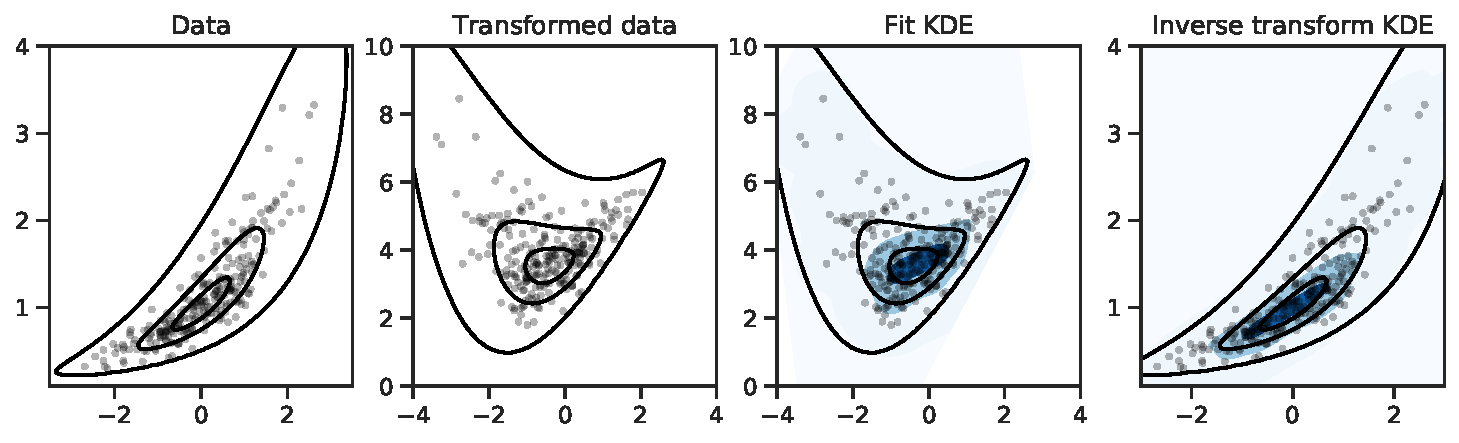
\includegraphics[width=0.9\textwidth]{figures/snemo_kde/2d_rescaling_process.pdf}
    \caption{The process of transforming the data to use a kernel that captures the data covariance. The first panel shows the data in the original coordinates. The second panel shows the data after being transformed by the whitening transformation. The third panel shows the KDE fit with a normal Gaussian kernel, and the final panel shows the data and the KDE reprojected back into the original coordinates. In each panel, the same data points are shown as black dots. The true 1, 2, and 3 $\sigma$ contours are shown in differing shades of blue. The black lines indicate the 1, 2, and 3 $\sigma$ confidence intervals of the best-fit KDE.}
    \label{fig:2d_rescaling_process}
\end{figure}

\begin{figure}
    \centering
    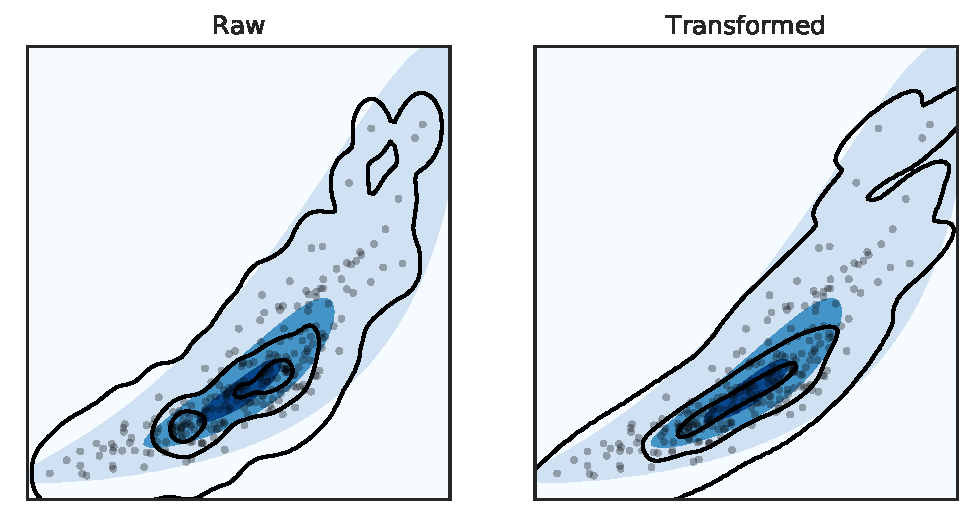
\includegraphics[width=0.9\textwidth]{figures/snemo_kde/2d_scatter.pdf}
    \caption{Comparison of the final KDE for our toy example using a) the best-fit Gaussian kernel with no covariance transformation and b) the best-fit Gaussian kernel with whitening applied. In both panels, the blue shading indicates the 1, 2, and 3 $\sigma$ contours of the true toy model distribution, and the black lines indicate similar contours for the kernel density estimates of the distribution.}
    \label{fig:2d_scatter_scaled}
\end{figure}

